
何谓算法? Wikipedia 中这样描述到
\begin{quotation}
	An algorithm is a finite sequence of well-defined, 
	computer-implementable instructions, 
	typically to solve a class of problems or to perform a computation.
\end{quotation}
算法始终是明确的,它是一个分步执行的过程,
该过程将一些值集作为其输入并生成一些值集作为其输出。
当然输入的值集需要满足一定条件,我们称之为先决条件(precondition)。
有了合理的输入以及明确的执行过程,
我们一定可以得到一个输出,即使有些时候这个输出并不是我们想要的,
我们称按照执行过程得到的结果满足的条件为后置条件(postcondition)。

有了前面这些概念,
我们可以把一个算法或者一个定理看做一个契约(contract)。
即
\textbf{你(用户)向我(开发者)提供满足先决条件的输入,
我将为你提供满足后置条件的输出}(如图 \ref{fig:contract} 所示)。
\begin{figure}[htbp]
	\centering
	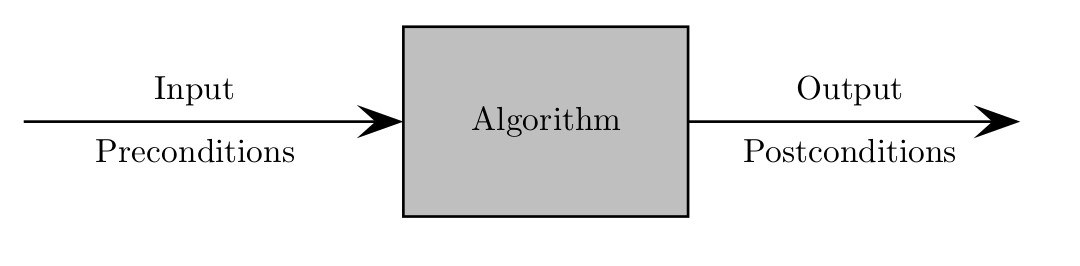
\includegraphics[width=0.8\textwidth]{png/contract}
	\caption{算法设计的契约。}
	\label{fig:contract}
\end{figure}
有了契约的概念,在算法设计的时候,明确算法的契约是非常重要的一步。
大到整个程序的框架,小至每个小模块的设计。
合理的算法契约在算法设计的时候不仅可以节省时间,
还可以让用户更快的了解该算法。

图 \ref{fig:bisection} 是求解非线性方程 $f(x)=0$ 时常用的二分法的算法契约。
其核心是每次将解的求解区间减半,直到近似解满足一定的条件。
输入中,$[a,b]$ 为算法开始给定的解的求解区间,$M$ 为最大的迭代次数,
$\epsilon, \delta $ 是两种不同的解的精度范围;
输出中, $c$ 是二分法得到的近似解,$h$ 是解所在的区间范围,
$k$ 为找到近似解所需要的迭代次数。
这里将二分法的具体实现看做一个黑盒子,
将细节忽略的好处是我们可以先更加专心的进行算法设计。
\begin{figure}[htbp]
	\centering
	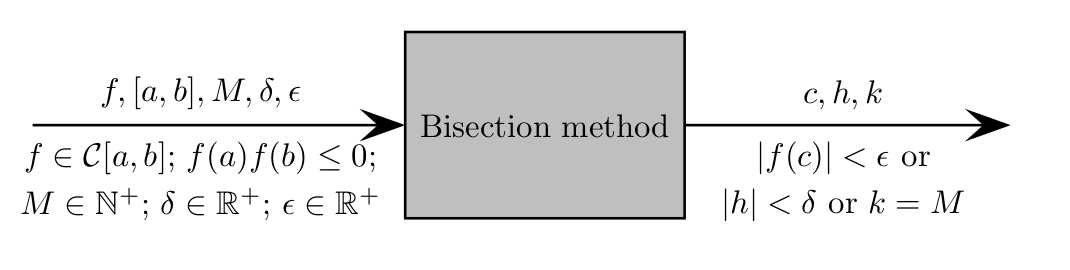
\includegraphics[width=0.8\textwidth]{png/bisectionMethod}
	\caption{求解非线性方程时常用的二分法的算法契约。}
	\label{fig:bisection}
\end{figure}
	
如果违反了先决条件,则该算法的行为或输出不确定。
为了确保先决条件,
我们要么在算法内部显式检查它们(关键字 \textbf{Check} 显示),
要么将此职责转移给用户(关键字 \textbf{Require} 显示)。 
在测试程序时,
实质上是在提供参数满足先决条件的测试用例后测试后置条件是否成立。


%%% Local Variables:
%%% mode: latex
%%% TeX-master: "../Guide"
%%% End:
